\documentclass[a4paper,12pt]{article}
\usepackage[utf8]{inputenc}
\usepackage[frenchb]{babel}
\usepackage{graphicx}
\usepackage[T1]{fontenc}
\usepackage{fancyhdr}
\usepackage{graphics}
\setcounter{page}{1}
\fancyhead[L]{\leftmark}
\fancyhead[R]{}

\fancyfoot[C]{}
\fancyfoot[R]{\thepage}


%PREMIÈRE PAGE / PAGE DE GARDE
\begin{document}
\begin{titlepage}
		\newpage
		\thispagestyle{empty}
		\begin{center}
			
\includegraphics[scale=0.1]{illustrations/logo-paris-nanterre}	
		\end{center}
		\begin{center}
			\vspace{0.3cm}
			\large  
			\textbf{Rapport de Stage Master 1 MIAGE classique}\\
			\vspace{0.7cm} \large 
			\vskip 0.2in
		\end{center}
		\fbox{%
			\parbox{\textwidth}{%
				\begin{center}
					\begin{center}
						\large \textsc{\textbf{Aide à la migration du contenu d'une base de données \\
						Création d'un système d'extraction de tweets}}
					\end{center}
					
				\end{center}
			}%
		}
		\begin{center}
		    
\includegraphics[scale=0.25]{illustrations/isover-logo}		
		\end{center}
		
		\begin{flushleft}
			\begin{center}
			    
			    \textbf{Auteur :}
				\hspace{0.1cm} William Piron \\
				\textbf{Lieu du stage :}
				\hspace{0.1cm}Isover, département BI\\
				\textbf{Tuteur en entreprise :}
				\hspace{0.1cm} Philippe Roulet \\
				\textbf{Tuteur enseignant :}
				\hspace{0.1cm} Emmanuel Hyon \\
							
			\end{center}
		\end{flushleft}
	
		\begin{center}
			\vspace{0.1cm} \textbf{9 Mai au 26 Août 2017}
		\end{center}
		
	\newpage



%REMERCIEMENTS
\thispagestyle{empty}
\section*{Remerciements}
Je remercie Isover de m'avoir accueilli au sein de sa structure dans le cadre de mon stage de fin d'année. \\
\indent Je tiens à remercier l'ensemble de l'équipe BI pour leur accueil chaleureux et leur aide. \\
\indent Enfin, je remercie particulièrement Philippe Roulet et Yann Berthaut pour leur temps, leur aide et leur confiance dans le cadre des projets qui m'ont été confiés.

%TABLE DES MATIERES
\newpage
\tableofcontents
\thispagestyle{empty}
\end{titlepage}
\newpage


\pagenumbering{arabic}
\addcontentsline{toc}{section}{Introduction}
\section*{Introduction}
Dans le cadre de ma première année de Master MIAGE au sein de l'Université Paris Ouest, j'ai effectué mon stage de fin d'année au sein d'Isover, entreprise du groupe Saint-Gobain.\\ \\

Durant les deux mois de stage effectué avant la rédaction de ce rapport, j'ai eu l'occasion de travailler sur deux projets. \\
\indent Le premier consistait à récupérer au sein des bases de données d'Isover des informations liées aux clients et aux ventes d'une entreprise rachetée par Isover et ne stockant pas ses données de la même manière. Le projet est actuellement en pause et est effectué sous la supervision de Yann Berthaut.\\ 
\indent Le deuxième projet consistait à mettre au point une application pouvant importer, via l'API Twitter, des tweets contenant des mots clés ou hashtag liés aux activités du groupe Saint-Gobain. Ce projet est actuellement en cours et est effectué sous la supervision de Philippe Roulet.\\ \\

Ce rapport présentera tout d'abord brièvement l'entreprise et le contexte professionnel du stage.\\
\indent Ensuite, pour chacun des projets sera détaillé son origine et contexte, les méthodes utilisées, et les éventuels changements apportés et difficultées rencontrées.


%PRESENTATION DE L'ENTREPRISE
\newpage
\addcontentsline{toc}{section}{Présentation d'Isover}
\section*{Présentation d'Isover}
\begin{center}
    
\includegraphics[scale=0.15]{illustrations/isover-logo}		
\end{center}
Fondée en 1936, Isover est une SA appartenant au pôle "Produit Pour la Construction (PPC)" du groupe Saint-Gobain.\\ \\

Leader mondial de l'isolation, l'entreprise propose de nombreuses solutions (isolation thermique, acoustique et protection feu), est implantée dans 39 pays et compte 9225 salariés dans le monde.\\

La vision de l'entreprise est centrée sur trois points :
\begin{itemize}
    \item Innover pour trouver toujours de nouvelles solutions
    \item Avoir la meilleur efficience énergétique possible
    \item Construire durablement dans le respect de l'environnement \\
\end{itemize}

\noindent L'équipe Business Intelligence (BI), au sein de laquelle j'ai effectué ce stage, est située au siège social de l'entreprise à Suresnes (92150). L'équipe travaille sur différent projets liés à d'autres organes du groupes et effectue également une mission de support aux utilisateurs de ses applications et solutions. \\ \\

C'est dans le ce cadre que s'inscrivent les deux missions qui m'ont été confiées lors de la première moitié de mon stage, détaillée dans ce rapport.

\begin{center}
    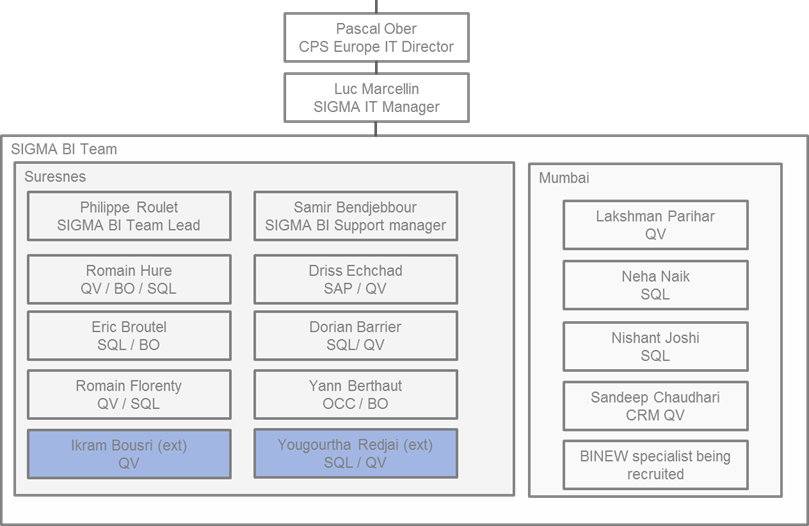
\includegraphics[angle=90, scale=0.9]{illustrations/organigramme-BI}

    Annexe 1 : Organigramme du département Bi de Suresnes
\end{center}



%PREMIER PROJET : MIGRATION DONNÉES D'UNE BASE DE DONNÉES
\newpage
\section{Projet Isonat}
\subsection{Présentation du projet}
\subsubsection{Origine}
Isonat (anciennement Buitex Recyclage) a été racheté en avril 2016 par Isover. Les deux sociétés ne stockant pas de la même manières leurs informations commerciales et liées à leur clients, un projet visant à importer et convertir les données d'Isonat chez Isover a été lancé.\\

Ce projet a été mis en pause puis relancé à l'occasion de mon arrivé dans l'entreprise, me permettant de le familiariser avec les outils et et le fonctionnement de la BI.


\subsubsection{Problématique et but}
Le but à terme de ce projet est simple : permettre une récupération des données de ventes réglées et livrées d'Isonat du dernier exercice comptable (révolu ou en cours), les mettre dans un format très proche de celui utilisé par Isover (à quelques absences d'informations près) puis stocker le tout dans les tables correspondantes de la base de données d'Isover.\\

Pour cela, il a été décidé de rédiger une procédure SQL récupérant les données sur le serveur Isonat et préparant localement une table au format d'Isover. Les données d'origine ne nécessitant pas de transformations sont mises directement dans les colonnes correspondantes de la table temporaire. \\
Certaines données ne sont pas dans le même format (notamment codes clients et produits) et nécessitent d'effectuer une correspondance via une table de mapping.\\
Dans le cas d'une donnée absente d'Isonat, non mappable et non essentielle, il a été décidé qu'une valeur par défaut (\# si texte, 0 si nombre) serait insérée à la place. \\

Enfin, les données traitées et reformatées doivent être insérées dans la table contenant les ventes à partir de la table temporaire.


\subsection{Développement et évolutions}
\subsubsection{Technologie utilisée}

\begin{center}
    
\includegraphics[scale=0.5]{illustrations/sql-server-icon.jpg}
\end{center}


Afin d'accéder à ses serveurs, l'équipe BI utilise le logiciel SQL Server Management Studio (SMSS).\\
SMSS est un environnement développé par Microsoft mis à disposition gratuitement permettant la gestion des infrastructures SQL. Il permet de configurer, surveiller et administrer des instances de SQL Server.\\
Ce logiciel  possède une version express gratuite qui comporte tout le nécessaire pour la réalisation de ce projet dans le cadre de mon stage. Le reste de l'équipe dispose de licences entreprise pour la version complète, qui dans mon cas n'apporte pas de réelle différence.\\

\begin{center}
    \hspace*{-0.22\textwidth}
    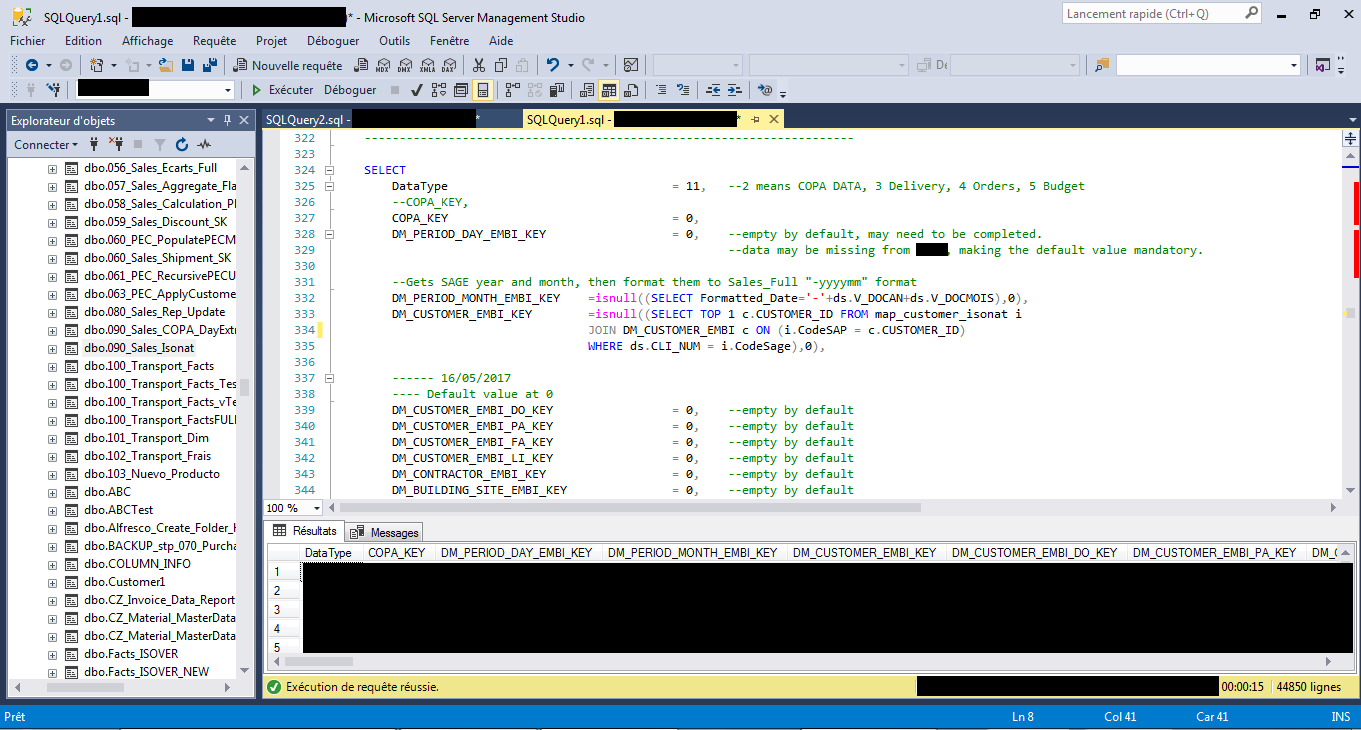
\includegraphics[scale=0.55]{illustrations/screen-smss-1}
    Par soucis de confidentialité, une partie des informations ont été noircies. \\    
    Annexe 2 : Capture d'écran SMSS
\end{center}


\subsubsection{Mise en œuvre}
Après plusieurs réunions avec Philippe Roulet et Yann Berthaut dans les premiers jours du stage, un accès sur les serveurs de développement et de production m'a été fourni, ainsi que sur le serveur Isonat, afin de commencer à appréhender le fonctionnement du logiciel et la logique des différentes bases sur les serveurs. \\
Il a été décidé que je créerai une procédure stockée SQL sur le serveur de développement, dont le fonctionnement serait basé sur d'autres procédures existantes (notamment l'insertion des données, en utilisant les bons noms de colonnes). La procédure a été rédigée par étape. \\
Il m'a également été fourni une liste de bonnes pratiques et méthodes à utiliser dans mon code, afin de rendre sa lecture et sa maintenance plus simple dans le futur dans le cas où un membre de l'équipe devrait le modifier. Cela inclut notamment un usage fréquent et correct de commentaires tout au long de la procédure, et la limitation au maximum des sous-requêtes afin d'alléger autant que possible la charge sur le serveur et le temps d'exécution. \\

Les deux premiers jours ont été dédié à la découverte de l'environnement de travail et de l'organisation des bases de données. Une fois tous les logiciels nécessaires installés, et la problématique et le but définis, la rédaction de la procédure a pu commencer. \\

\subsubsection{Points clés du projet}
Le but final de la procédure étant de faire le lien entre les activités de la filiale Isonat et de sa maison mère Isover, il est essentiel que les données clés soit bien identifiées, afin que leur transfert d'une entité à l'autre se fasse de manière efficace. \\

Les codes essentiels à transmettre à Isover sont les identifiants clients et produits, enregistrés différemment par les deux entités. Il est impératif qu'une correspondance puisse se faire. Si ce n'est pas possible, c'est à dire si un code client ou produit n'est pas présent dans les catalogues de données d'Isover, il faut que l'information soit créée, ou à défaut mappée avec un code regroupant les données inconnues dans une seule catégorie.

\subsubsection{Étapes de développement} 
Avant mon arrivée sur ce projet, un premier jet de requête de récupération des données sur le serveur avait été fournie par la cellule métier. Elle a peu évoluée lors du développement, mais a été complétée afin de soit récupérer l'ensemble des données de vente (si inexistante sur le serveur de développement), soit uniquement les plus récentes (année précédente et en cours) afin de mettre à jour la base. \\
Cette requête récupère à partir des différentes tables du serveur l'ensemble des données estimées comme utiles par la cellule métier, notamment les articles vendus, les clients, les montants et les dates de vente. Le résultat comporte 27 colonnes extraites tel quel, certaines nécessitant un léger traitement par la suite. \\
Cette requête représente le plus gros de la procédure, et les données obtenus grâce à elle sont essentielles. Les quelques modifications de format de données nécessaire à la suite de la procédure ont été réalisées sur son résultat plutôt que dans la requête. Cela a permit de limiter au maximum de fausser l'extraction.\\

Ensuite, le corps principal de la procédure, c'est à dire la partie permettant le mapping des données, a été complété. Une bonne partie des données ont pu être utilisées directement, en les plaçant dans les colonnes correspondantes, mais certaines ont du subir des transformations.\\
Les dates ont subi un changement de format légers, de nombreuses colonnes ont reçu des valeurs par défaut comme décidé, puis un mapping temporaire (incomplet) a été réalisé à partir de fichiers obtenus auprès du métier.Ceux ci contiennent les codes articles et les codes clients utilisés par Isonat et leur correspondance vers ceux utilisés par Isover. Dans le cas où l'équivalence est inconnue, un code "divers" a été défini après concertation avec le métier,et utilisé pour combler les informations manquantes. \\
La table finale comporte 174 colonnes. Seule une quinzaine peut être obtenue à partir des données extraites et des mappings. Une très grande partie ne peut pas être déterminée à cause de la différence de traitement des commandes entre les deux entités (notamment les étapes intermédiaires de facturation) ou par une absence de correspondance. Comme précisé dans la problématique, toutes ces informations reçoivent une valeur par défaut.


\subsubsection{Ajouts et initiatives}
En discutant avec mon tuteur lors d'un point sur l'avancement du projet, il m'a suggéré d'importer uniquement les données les plus récentes afin de minimiser la charge sur le serveur (bien qu'assez faible), en se basant sur la date d'exécution. L'idée était de ne mettre à jour qu'au plus la tranche allant de l'année N-1 à l'année en cours, voire moins si la date d'extraction est assez avancée dans l'année en cours. \\

J'ai donc implémenté une vérification de date lors du lancement de la procédure, ainsi qu'une vérification de l'existence de la table recevant les données importées non traitées. Dans le cas où la table n'existe pas, l'import a lieu sans condition de date et concerne toutes les données de ventes Isonat. Dans le cas contraire, et en cas d'exécution avant le mois de mars de l'année en cours, on importe l'année N et N-1. Sinon, on importe uniquement l'année N.\\
Cela permet de récupérer uniquement le plus récent et le plus utile au métier lors de l'exécution, et de garder les données à jour. Les données de l'année N-1 sont écrasées si l'exécution a lieu avant mars, afin de prendre en compte d'éventuels changements depuis la fois précédente, et sont juste complétées dans le cas contraire.\\

De plus, un bloc de transaction a été mis en place autour de la requête d'import afin de bloquer l'accès à la table intermédiaire et d'éviter une suppression des données en cas d'erreur. Cela permet une meilleure sécurité des données sans pour autant bloquer une table cruciale au travail des autres utilisateurs. \\
Enfin, suite à des erreurs de collation des données au format texte, un ensemble d'"ALTER TABLE" a été placé dans la transaction pour que les données temporaires soient directement dans un format identique aux données Isover, afin d'éviter une conversion donnée par donnée dans la suite de la procédure.\\
Divers légères optimisations ont été effectuée, notamment l'ajout d'une limitation "TOP 1" dans les sous-requêtes utilisés lors des mappings clients et articles.\\

\begin{center}
    \hspace*{-0.22\textwidth}
    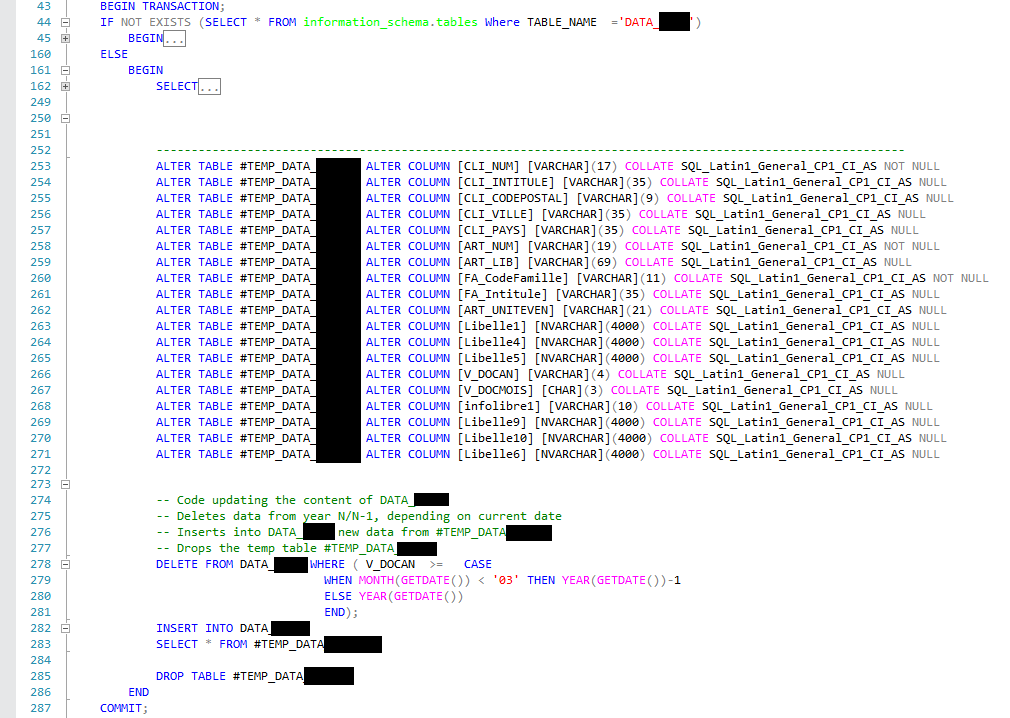
\includegraphics[scale=0.75]{illustrations/screen-smss-2}
    Par soucis de confidentialité, une partie des informations ont été noircies ou cachées. \\
    
    Annexe 3 : Capture d'écran de la transaction
\end{center}


\subsection{Futur du projet}
Actuellement, le projet est en attente des fichiers de mapping finaux afin d'obtenir une correspondante complète entre les codes articles et clients de Isonat vers leur équivalent Isover.\\

La version actuelle de la procédure effectue la quasi-totalité des opérations que la version finale du projet doit faire, et ne devra normalement subir que quelques petites modifications une fois les fichiers de correspondance complets. Certaines données seront sans doute complétées en fonction des besoins du métier au cas par cas.\\

A terme, la procédure sera lancé régulièrement afin de prendre en compte l'évolution des ventes Isonat (notamment l'état des commandes) et permettra de maintenir à jour de manière fiable le montant de ventes de l'entreprise. \\

Le second projet détaillé dans ce rapport a été mis en route afin de combler cette période d'attente. Il n'est pas exclu qu'il soit lui même mis en pause lorsque les informations manquantes seront transmises, puis repris dès que la procédure SQL aura été validée et passée en production.




%SECOND PROJET : EXTRACTION DE TWEETS
\section{Projet d'extraction de tweets}
\subsection{Présentation du projet}
\subsubsection{Origine}
L'idée de ce projet est née d'une discussion avec le service marketing, évoquant la possibilité dans une futur proche de vouloir effectuer des tableaux de bords sur ces données. Il s'agissait d'un point abordé à plusieurs reprises lors de différentes discussions avec l'équipe BI, sans être un point central de celles ci. Il s'agissait davantage d'évoquer une nouvelle analyse de données pouvant être ajoutée aux outils existant.\\

La BI a donc lancé en anticipation un projet visant à extraire des données depuis Twitter. Les tweets mentionnant les activités du groupe Saint-Gobain, plus spécifiquement celles des entreprises Isover, Placo et Weber, seraient récupérés. Ils seraient ensuite analysés selon plusieurs critères afin de fournir des chiffres exploitables et utiles au service marketing. \\
A ce stade du projet, seul Philippe Roulet travaillait dessus en parallèle de ses projets principaux et de ses activités de gestion de l'équipe BI.


\subsubsection{Problématique et but}
Afin de pouvoir obtenir des informations exploitables depuis les tweets extraits, il a fallu en déterminer les données clés à extraire :
\begin{itemize}
    \item Les hashtags utilisés, pour déterminer le contexte du tweet
    \item Le nombre de retweets et de "j'aime", pour connaître sa portée
    \item Son texte, pour obtenir un maximum d'information
    \item La "sensibilité", pour savoir s'il est vulgaire ou offensant et ne pas en tenir compte
\end{itemize}
Le but est de pouvoir déterminer des tendances concernant les marques du groupe Saint-Gobain, savoir si les utilisateurs et clients en parle, et comment. \\
Ces informations permettront de faire différents graphiques utilisables par le service marketing pour tirer différentes conclusions concernant l'image et la popularité des produit par exemple.


\subsection{Développement et évolutions}
\subsubsection{Récupération de l'existant}
Lors de la réunion de lancement du projet, Philippe Roulet m'a expliqué qu'il avait commencé à travailler de son coté sur le sujet, et avait choisi de s'orienter sur une application Python utilisation l'API Twitter dédiée, ainsi qu'une base de donnée NoSQL MongoDB. Pour cela, il m'a fourni la machine virtuelle Ubuntu sur laquelle il avait travaillé, et contenant les logiciels PyCharm et MongoBooster.\\

PyCharm est un IDE Python développé par JetBrains permettant une meilleure organisation des fichiers au sein de l'arborescence du projet, et comportant bon nombre de raccourcis et outils facilitant le développement.\\
MongoBooster est un outil graphique multi-plateforme pour MongoDB contenant un constructeur de requête et une aide syntaxique. Il permet une manipulation plus fluide des bases MongoDB ainsi qu'une meilleur visualisation des données. \\

\begin{center}
    
\includegraphics[scale=0.5]{illustrations/pycharm-mongodb-logo}
\end{center}

La simplicité du Python permettait d'écrire simplement mais efficacement un programme permettant l'import de tweets localement, en se connectant à Twitter via l'API Tweepy, pour ensuite stocker dans la base NoSQL. \\
La connexion se fait via une compte Twitter (il est donc obligatoire de s'y inscrire), en créant ensuite une application Twitter. Une fois l'application créée, le compte se voit attribué une clé d'utilisateur, une clé privée, un jeton d'accès et un jeton privé. C'est à partir d'eux que la connexion entre l'application Python et Twitter se fait.\\
Une fois l'accès obtenu via l'API, il suffit d'importer la librairie Tweepy pour effectuer des requêtes sur l'ensemble des tweets, en précisant de nombreux paramêtres en fonction de nos besoins. \\

Le choix de la base NoSQL s'explique par la facilité de stocker un tweets dans un environnement de ce type, leur structure étant assez compliquée : beaucoup de champs, tableaux de tableaux, etc. Cela rend leur stock dans une base relationnelle très difficile, tout comme l'exploitation de certains champs. La grande taille et le grand nombre de champs de chaque tweets ajouterait également un grand nombre de dépendances et de jointures s'ils étaient stockés dans une base relationnelle plus classique.

\begin{center}
    \hspace*{-0.22\textwidth}
    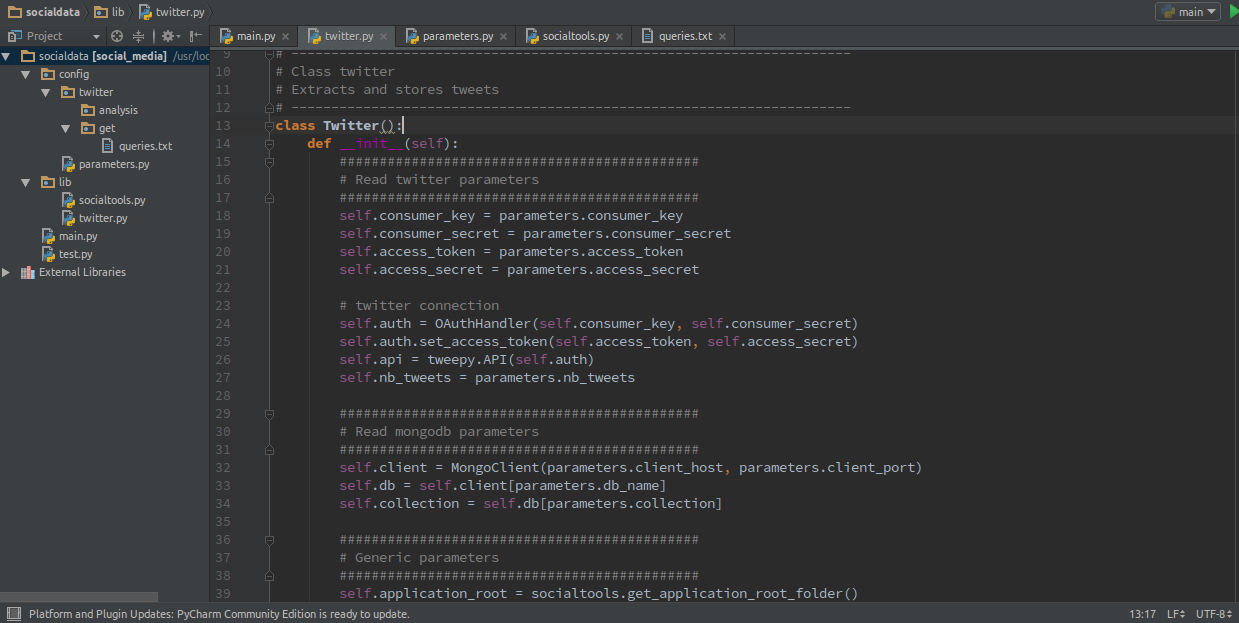
\includegraphics[scale=0.6]{illustrations/python-screenshot}
    
    Annexe 4 : Capture d'écran du code Python
\end{center}


\subsubsection{Problèmes soulevés et changements}
Une fois PyCharm et MongoBooster pris en main, j'ai commencé à travailler sur le sujet en analysant la structure des tweets et le système de requête de la base NoSQL. Outre la limitation du nombre de tweets maximum que l'API extrait à la fois, un autre problème s'est rapidement soulevé.\\
Là où les requêtes sur une base SQL relationnel permettent d'extraire un ensemble de tuples basé sur un filtre assez large, MongoDB force la présence explicite d'une condition. Par exemple, à la place d'une clause "WHERE xxx NOT NULL", MongoDB force la comparaison du champs à une valeur fixe. \\
En plus de cela, la structure même des tweets stockés risquait de rendre long et compliqué la récupération des hashtags utilisés, ceux-ci stockés dans des sous-tableaux de sous-tableaux. \\

Après plusieurs recherches, comparaisons et tests, j'ai décidé de me tourner vers l'utilisation de scripts R depuis le logiciel GNU R, disponible sous Windows. \\

\begin{center}
    
\includegraphics[scale=0.25]{illustrations/r-logo}
\end{center}

R est un langage dédié aux statistiques et à la science des données. Il implémente notamment de nombreux outils statistiques et graphiques dédiés à l'analyse de données, accrus par la multitude librairies et extensions disponibles. \\

Avant de changer de structure et de langage, une réunion a été organisée avec Philippe Roulet. Après discussion et explications, le changement de structure et de langage a été validé. Il s'était dégagé de l'entretien que même si les choix de bases semblaient parfaitement adaptés, les problèmes liés à l'utilisation des données extraites justifiaient le changement et la mise en place d'une nouvelle solution.


\subsubsection{Mise en œuvre}
Afin de rédiger mes scripts et requêtes R, je me suis dirigé vers GNU R, déjà utilisé en cours de statistiques lors du semestre 2 de cette année, gratuit et facile d'utilisation. Après la lecture de différents guides sur l'import de données depuis Twitter, et de mon cours de statistiques sur l'utilisation de R, je me suis lancé dans le projet à proprement parler. \\

En premier lieu, j'ai rédigé un script de connexion. Celui-ci importe et installe les librairies "twitteR" et "ROAuth", qui contienne le nécessaire à la connexion, puis se connecte au compte Twitter dont les clés et jetons sont stockés dans des variables. Celles-ci sont le seul élément du script à modifier en cas de changement de compte. \\

\begin{center}
    \hspace*{-0.23\textwidth}
    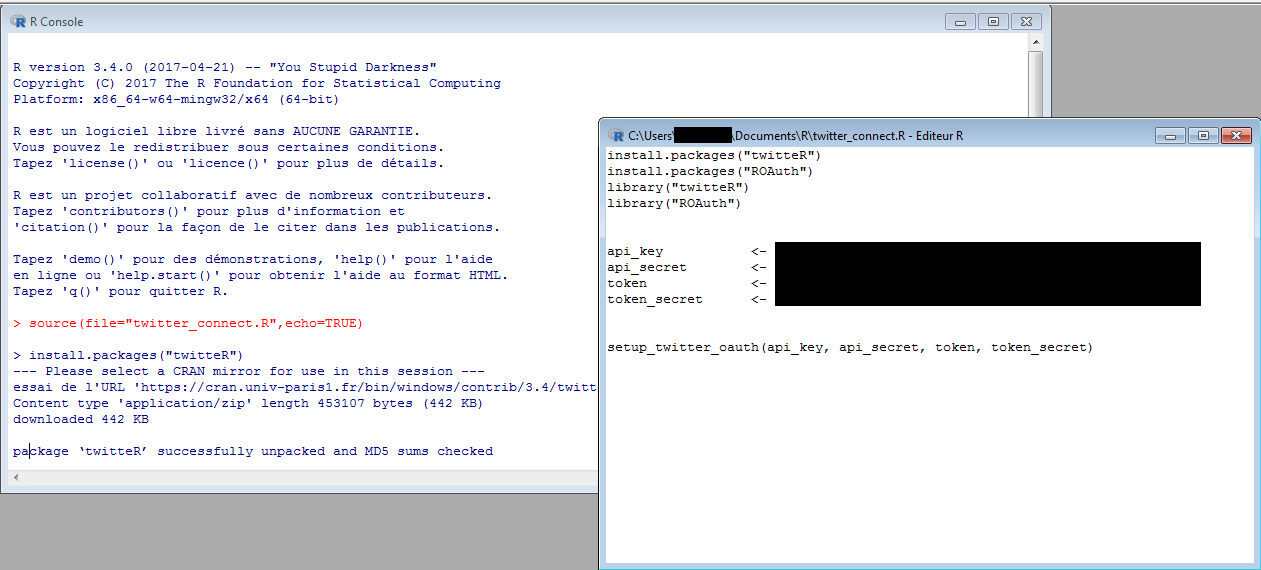
\includegraphics[scale=0.6]{illustrations/r-script-screen}
    Par soucis de confidentialité, une partie des informations ont été noircies. \\
    
    Annexe 5 : Capture d'écran de GNU R incluant le script de connexion
\end{center}


Une fois la connexion effectuée, il suffit de stocker dans une variable le résultat de la commande "searchTwitter", qui permet une recherche basée sur de nombreux critères. La plupart du temps, la recherche ne nécessite pas plus que les quatre arguments suivants :
\begin{itemize}
    \item searchstring : les chaînes ou hashtag à rechercher dans le texte des tweets, à séparer par OR ou + au sein d'une chaîne de caractères
    \item n : le nombre maximum de tweets à importer
    \item lang : la langue sur laquelle restreindre la recherche
    \item since : la date à partir de laquelle importer
\end{itemize}
La variable contenant désormais le résultat de la requête, il faut l'enregistrer en dur dans un document pour pouvoir la visualiser facilement. \\
Un second script a donc été rédigé : il exécute une requête, converti le résultat en data frame, puis stocke celle-ci dans un fichier csv.\\

\begin{center}
    \hspace*{-0.17\textwidth}
    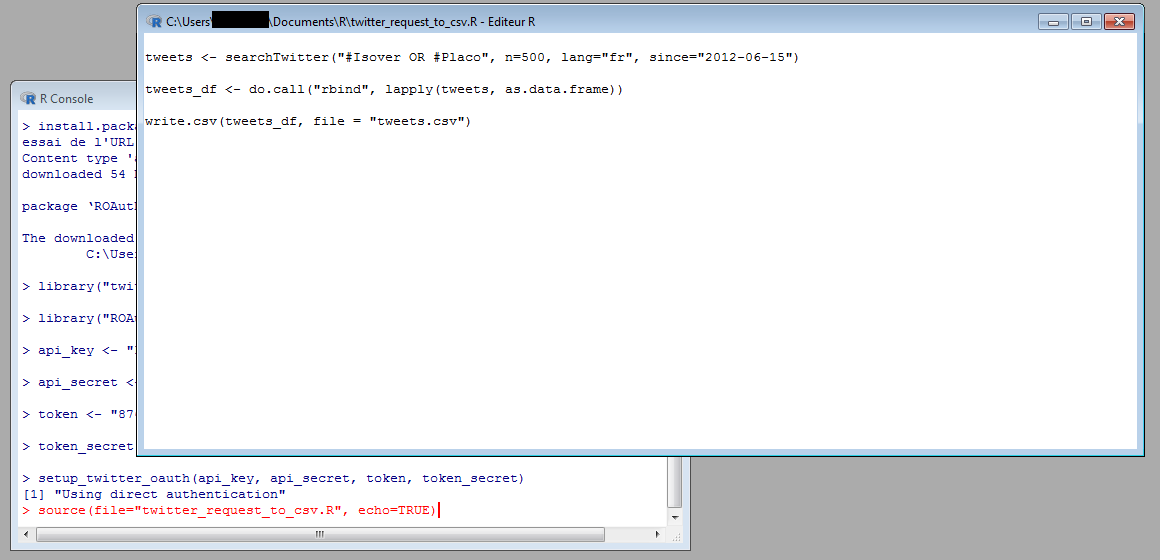
\includegraphics[scale=0.6]{illustrations/r-script-screen-2}
    Par soucis de confidentialité, une partie des informations ont été noircies. \\
    
    Annexe 6 : Script de requête R avec exemple de requête à quatre arguments
\end{center}


\subsection{Futur du projet}
Au moment de la rédaction de ce rapport, le projet est toujours en cours d'évolution et de réalisation. \\

A terme, le fichier .csv de sorti actuel sera très probablement remplacé ou complété par un fichier .pdf contenant divers graphiques ou courbes. \\
Le paramétrage actuel est extrêmement limité, forçant l'édition des script pour modifier les informations de compte Twitter ou la requête à exécuter. Une solution serait de rajouter un système de saisie manuelle des arguments ou un fichier de paramétrage unique lu par les scripts lors de leur exécution.\\

De même, l'obtention d'une licence SQL Server 2016 et son installation pourrait faciliter le fonctionnement du projet et de l'application ou du script final. En effet, le logiciel inclus un support R et Python, tout en permettant un stock dans une base relationnel. Seul soucis empêchant actuellement son installation, il n'est pas disponible pour les versions de Windows antérieurs à 8, ce qui est le cas de la grande majorité des postes du département BI.\\

Enfin, une autre piste d'évolution serait de rendre l'interface et l'extraction en elle même davantage "user friendly" que l'invité de commande de base de GNU R. Cela n'est pas le plus important, mais pourrait représenter un plus.


% CONCLUSION DU RAPPORT
\newpage
\addcontentsline{toc}{section}{Conclusion}
\section*{Conclusion}
Pour conclure ce rapport, j'aimerai une fois de plus remercier l'ensemble de l'équipe BI d'Isover, ainsi que toutes les personnes travaillant dans les autres services de l'entreprise avec lesquels j'ai eu l'occasion de travailler. Ils ont toujours pris le temps de répondre à mes questions ou de m'aider lors de mon travail sur mes projets, et m'ont permis de m'intégrer rapidement au sein du département.\\

Ce stage m'a permis de découvrir une nouvelle facette de l'entreprise, qui en plus d'être très intéressante, m'a donné des pistes sérieuses dans mon orientation future. Le domaine de la Business Intelligence, en plus d'être une voie d'avenir au sein des entreprises, m'a donné envie de m'y plonger davantage et à renouvelé ma motivation pour les années à venir.\\

J'ai pu mettre en pratique des connaissances et compétences diverses acquises pendant ma formation, ainsi que découvrir de nouvelles choses afin de les étendre.\\

La confiance de mon tuteur Philippe Roulet ainsi que sa disponibilité pour répondre à mes interrogations ont rendu l'expérience de ce stage d'autant plus agréable et m'ont donné la sensation d'être un composant de l'équipe à part entière.\\

Je ressors de ce stage extrêmement satisfait de mon expérience, et attend avec impatience de voir ce que les deux prochains mois au sein de l'entreprise peuvent encore m'apporter.

\end{document}
